\documentclass[a4paper, brazil]{article}
\usepackage[utf8]{inputenc}

\usepackage[cm]{fullpage}
\usepackage{pacotesLaTeX}

\author{Thales Freitas Macêdo \\ DRE: 115 162 177}
\title{LISTA 5}

\begin{document}

\maketitle

\section{Exercício 1}

\subsection*{1.a)}

    \begin{figure}[ht]
        \centering
        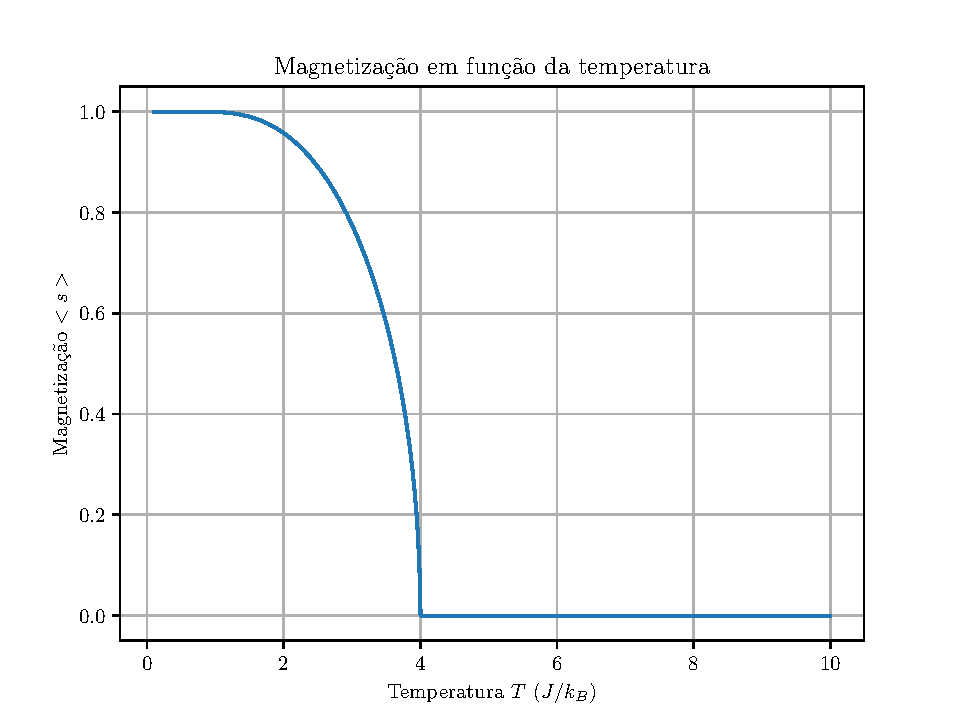
\includegraphics[width=0.7\textwidth]{fig_1a.pdf}
        \caption{Gráfico da magnetização em função da temperatura, pela solução da equação de campo médio do modelo de Ising na rede quadrada.}\label{fig1a}
    \end{figure}

    Para resolver numericamente a equação
    \begin{equation}
        \expval{s} = \tanh( \frac{z J \expval{s}}{\kB T} )
    \end{equation}
    usei o método de Newton-Raphson.
    Esse método consiste em aproximar a raíz de uma função \( f(x) \) pela raíz \( x_1 \) da reta tangente a \( f \) em uma primeira aproximação \( x_0 \) da raíz.
    Esse processo pode ser repetido, obtendo a fórmula iterativa
    \begin{equation}
        x_{i + 1} = x_{i} - \frac{f(x_i)}{f'(x_i)}
    \end{equation}
    que expressa a aproximação \( x_{i + 1} \) em termos da aproximação \( x_i \) anterior.

    Para isso considerei a função
    \begin{equation}
        f(\expval{s}) = \expval{s} - \tanh( \frac{z J \expval{s}}{\kB T} ) ,
    \end{equation}
    cujas raízes são as soluções desejadas.
    Para a rede quadrada, o número de primeiros vizinhos é 4, e portanto \( z = 4 \).
    Considerei \( J > 0 \) e expressei a temperatura em unidades de \( J / \kB \).
    Assim, encontrei a raíz positiva não-trivial de \( f (\expval{s}) \) para múltiplos valores de \( T \), compreendidos entre 0 e 10.

\newpage
\subsection*{1.b)}

    \begin{figure}[ht]
        \centering
        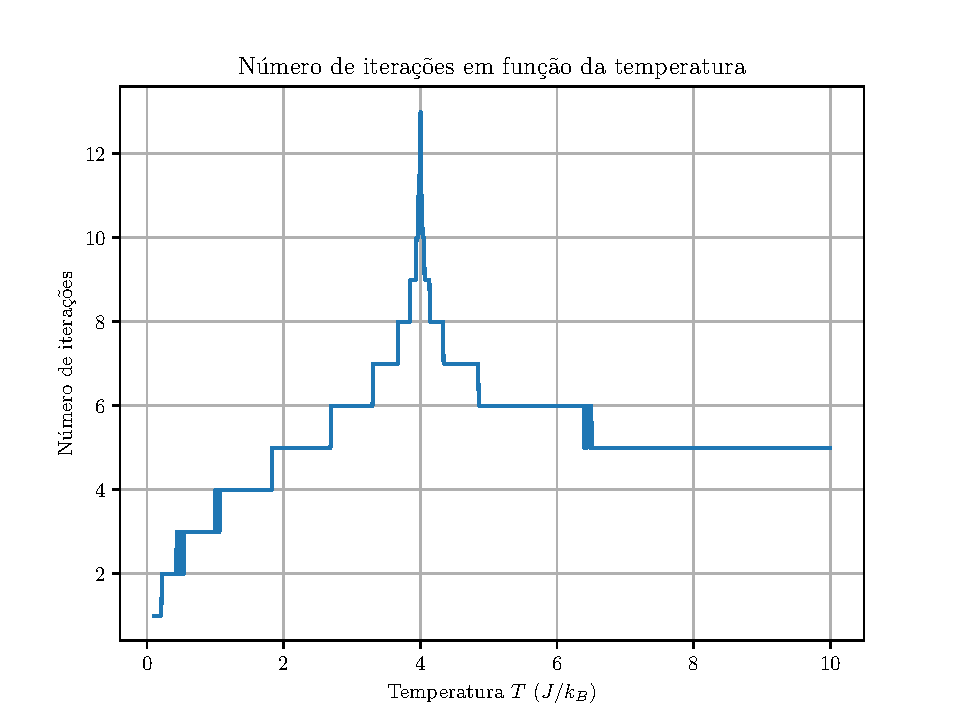
\includegraphics[width=0.7\textwidth]{fig_1b.pdf}
        \caption{Gráfico do número de iterações em função da temperatura do item anterior.}\label{fig1b}
    \end{figure}

    Para obter as soluções do item anterior, usei a aproximação inicial
    \begin{equation}
        \expval{s}_0 = 5
    \end{equation}
    e a condição necessária para o término das iterações
    \begin{equation}
        \abs{f( \expval{s}_{i + 1} )} < \num{1e-8} .
    \end{equation}

\newpage
\subsection*{1.c)}

    \begin{figure}[ht]
        \centering
        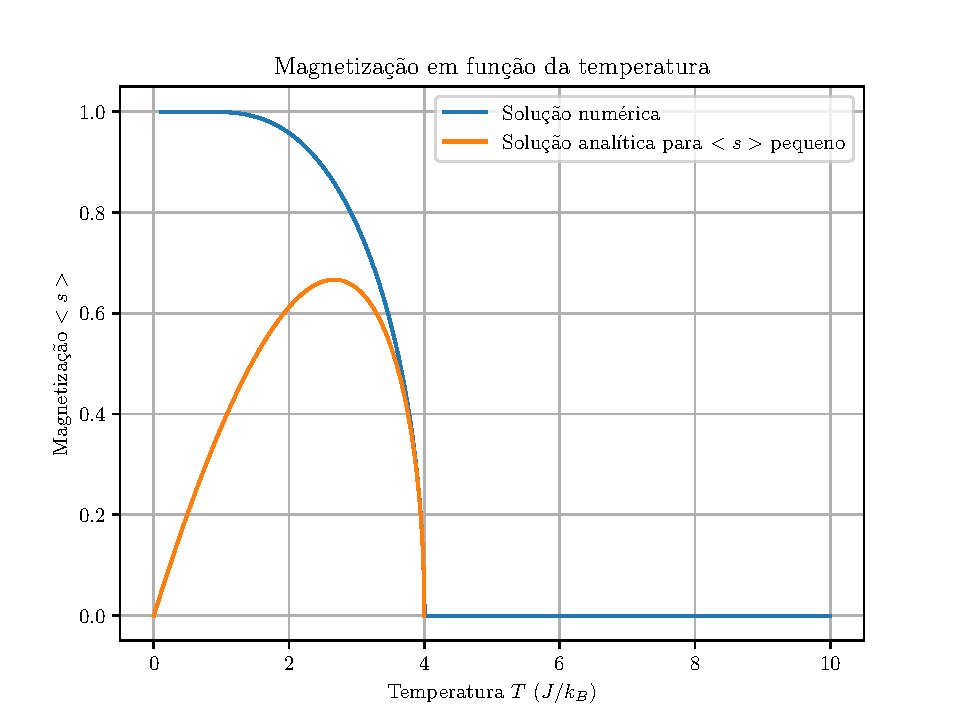
\includegraphics[width=0.7\textwidth]{fig_1c.pdf}
        \caption{Gráfico da magnetização em função da temperatura.}\label{fig1c}
    \end{figure}
    
    A solução analítica para pequenos valores de \( \expval{s} \) é adequada somente para valores de \( T \) próximos ao valor crítico \( T_c = 4 \).

\newpage
\subsection*{1.d)}

    Para a rede cúbica, a única diferença é que \( z = 6 \).
    Assim, os resultados são quase idênticos aos anteriores.
    \begin{figure}[ht]
        \centering
        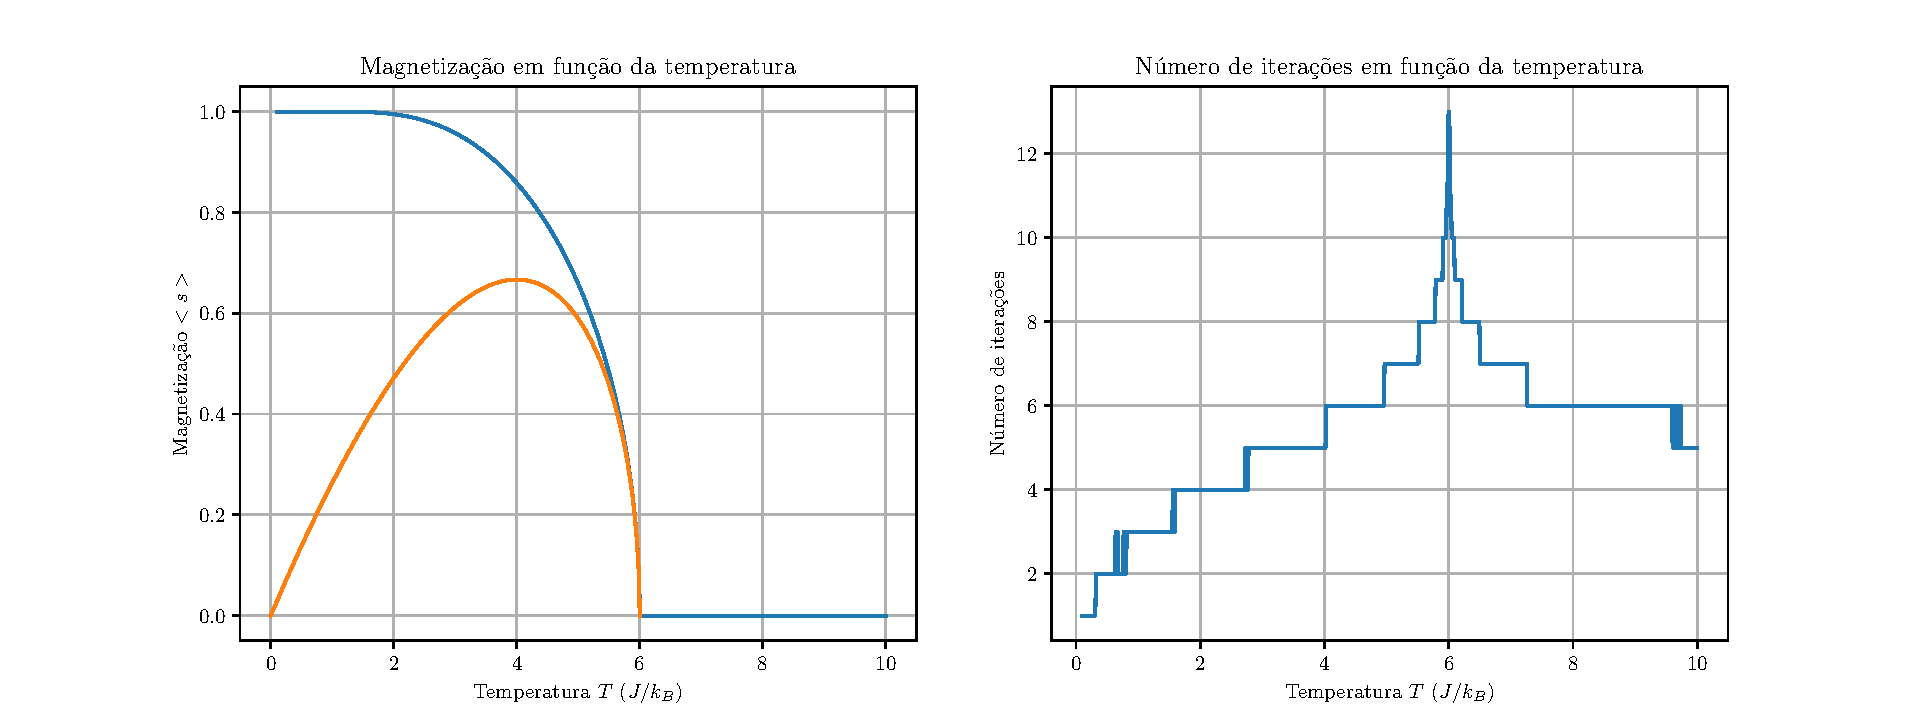
\includegraphics[width=\textwidth]{fig_1d.pdf}
        \caption{Gráfico da magnetização em função da temperatura.}\label{fig1d}
    \end{figure}

\newpage
\section{Exercício 2}

\subsection*{2.a)}

    \begin{figure}[ht]
        \centering
        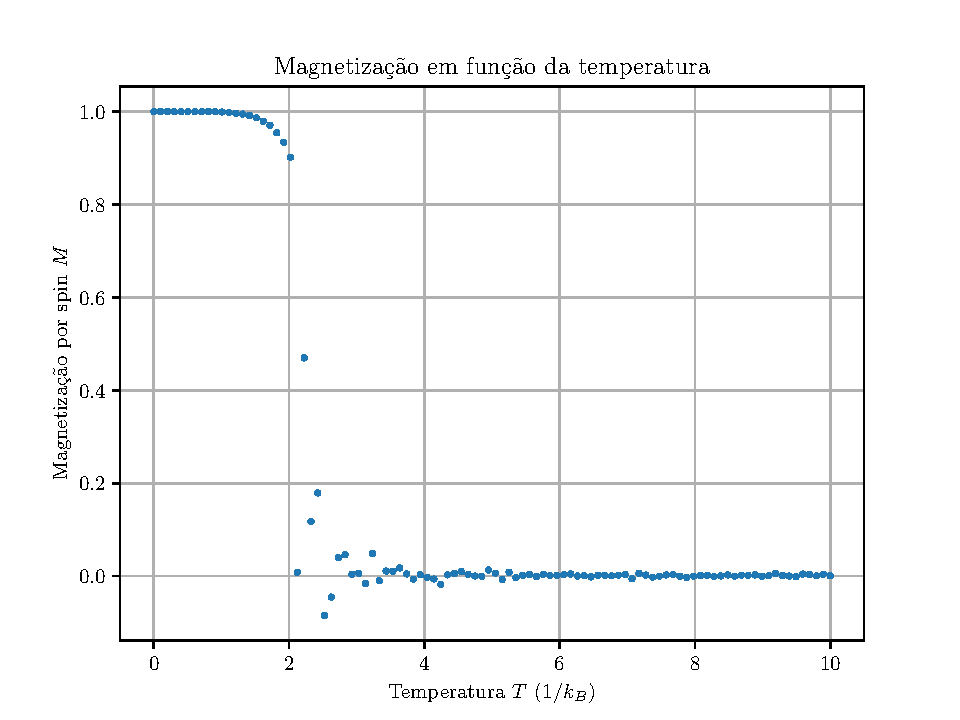
\includegraphics[width=0.5\textwidth]{fig_2a.pdf}
        \caption{Gráfico da magnetização em função da temperatura.}\label{fig2a}
    \end{figure}

    \begin{figure}[ht]
        \centering
        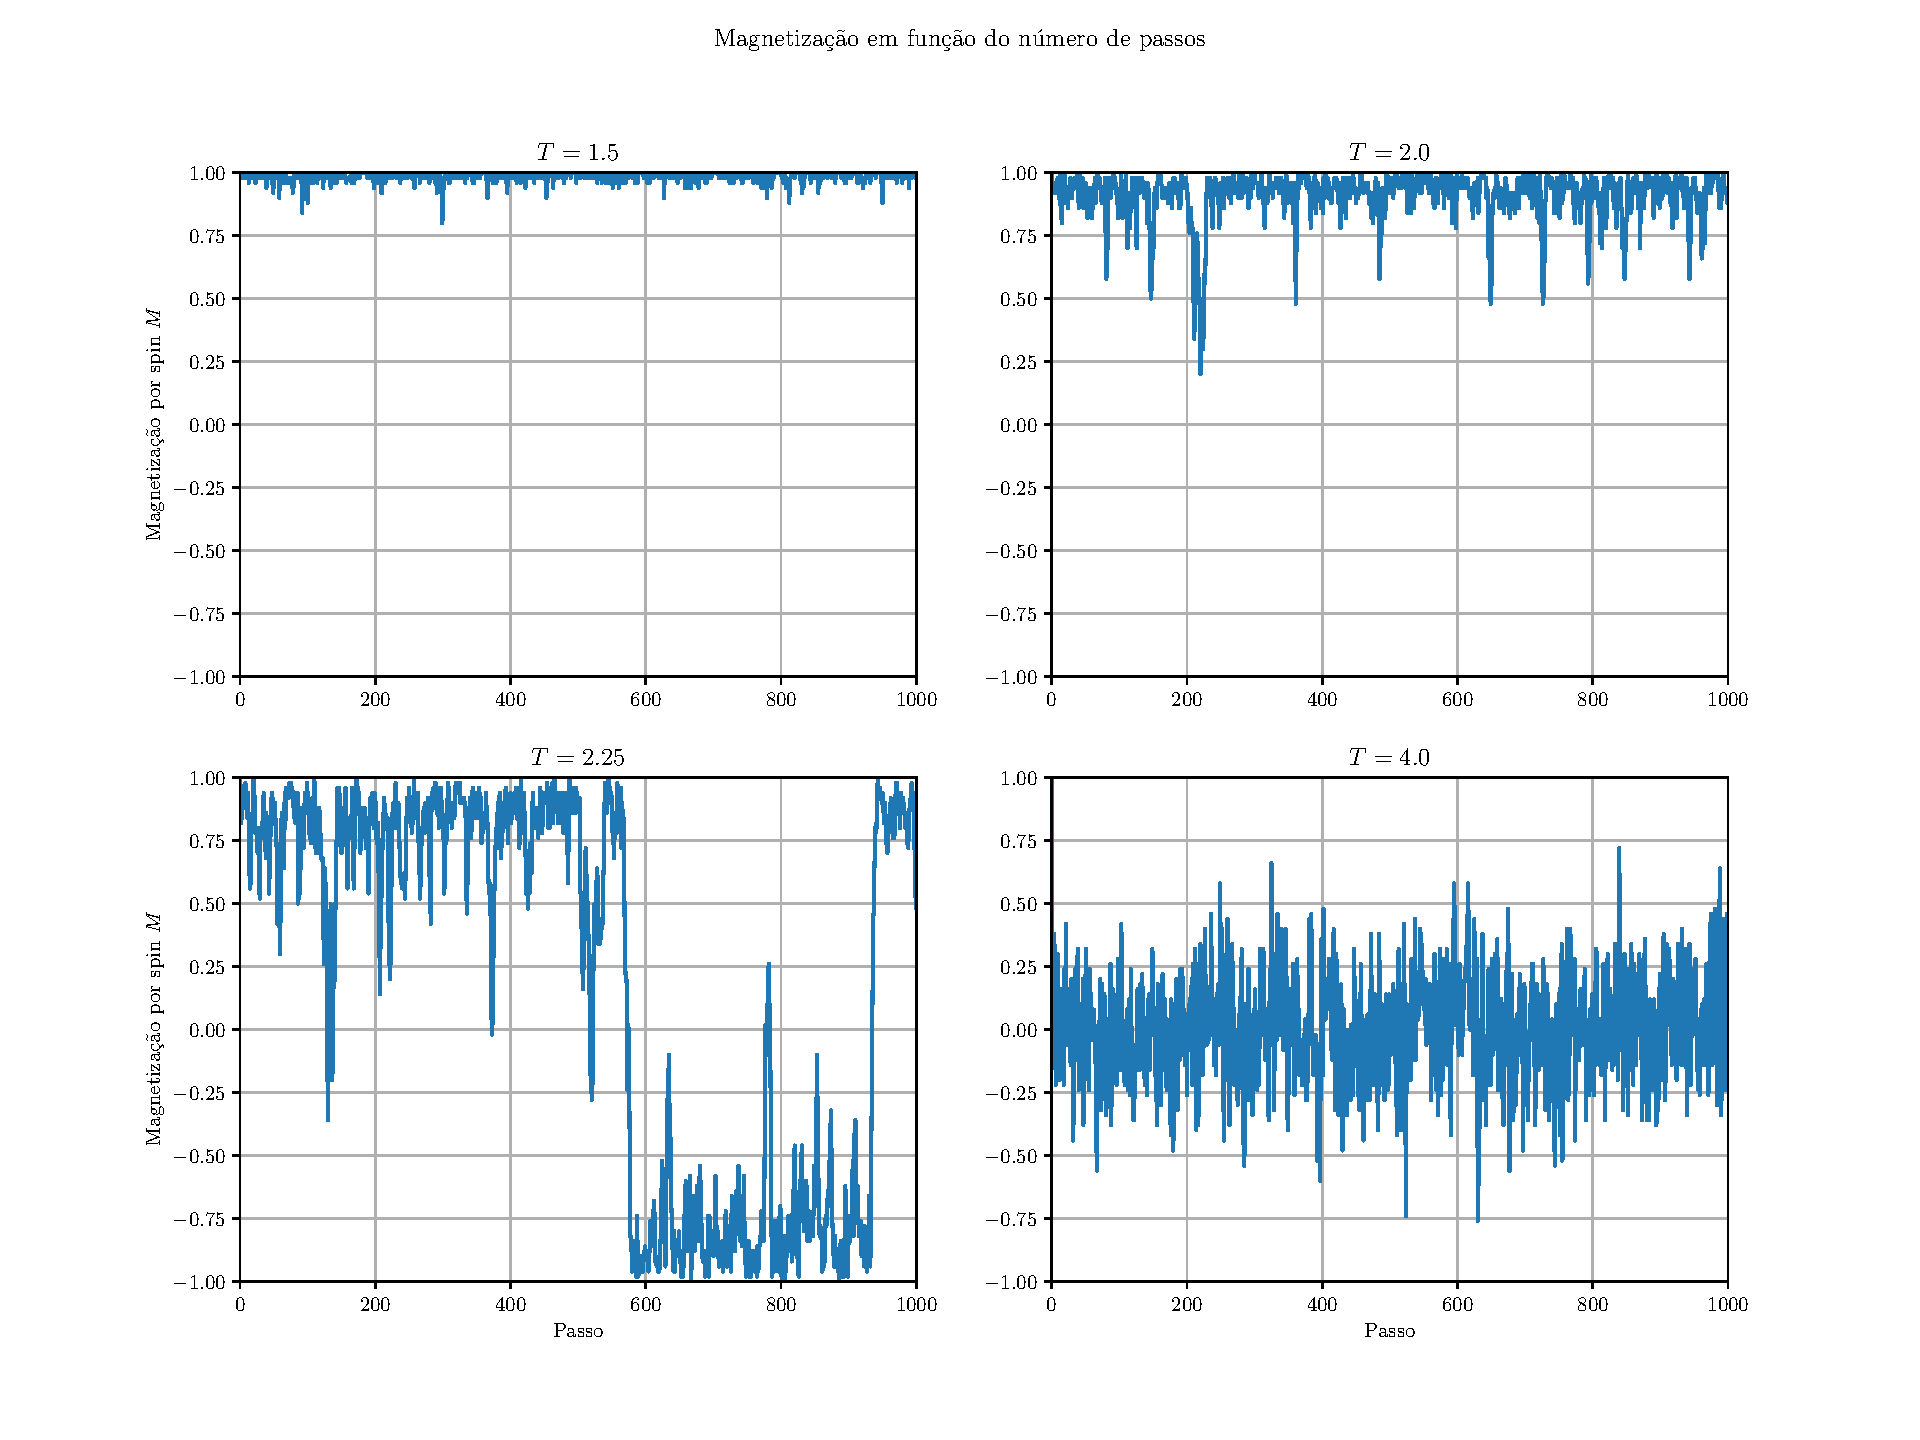
\includegraphics[width=0.5\textwidth]{fig_2a2.pdf}
        \caption{Gráfico da magnetização em função do número de passos.}\label{fig2a2}
    \end{figure}

    Para calcular a magnetização, usei o algoritmo de Metropolis para uma rede \( 10 \times 10 \) e um tempo de simulação de 1000 passos.
    Começo com um array \( 10 \times 10 \), com todos os valores iguais a 1, representando os spins.
    Escolho um valor para a temperatura.
    Assim, inicio um passo, que consiste em varrer a rede de spins, coluna por coluna.
    Para cada spin, determino a energia \( E_0 \) da rede, usando a fórmula
    \begin{equation}
        E = - J \sum_{\expval{i j}} s_i s_j ,
    \end{equation}
    e a energia da rede caso o spin estivesse invertido, \( E_1 \), determino a energia necessária para trocar o spin, \( E_\text{flip} = E_1 - E_0 \).
    Uso condições de contorno periódicas, de modo que considero interações entre os spins da primeira e última colunas, e interações entre os spins da primeira e última linhas.
    Se a energia \( E_\text{flip} \leq 0 \), eu troco o spin de orientação.
    Se a energia \( E_\text{flip} > 0 \), eu gero um número aleatório \( r \) entre 0 e 1.
    Faço então uma comparação de \( r \) com o fator de Boltzmann da energia \( E_\text{flip} \).
    Se \( r \leq \exp( - E_\text{flip} / \kB T) \), eu troco o spin de orientação.
    Caso contrário, eu o mantenho com a mesma orientação.
    Assim eu gero a rede de spins para o passo seguinte.
    Repito o procedimento para o número de passos desejado, no caso 1000.


\newpage
\subsection*{2.b)}

    \begin{figure}[ht]
        \centering
        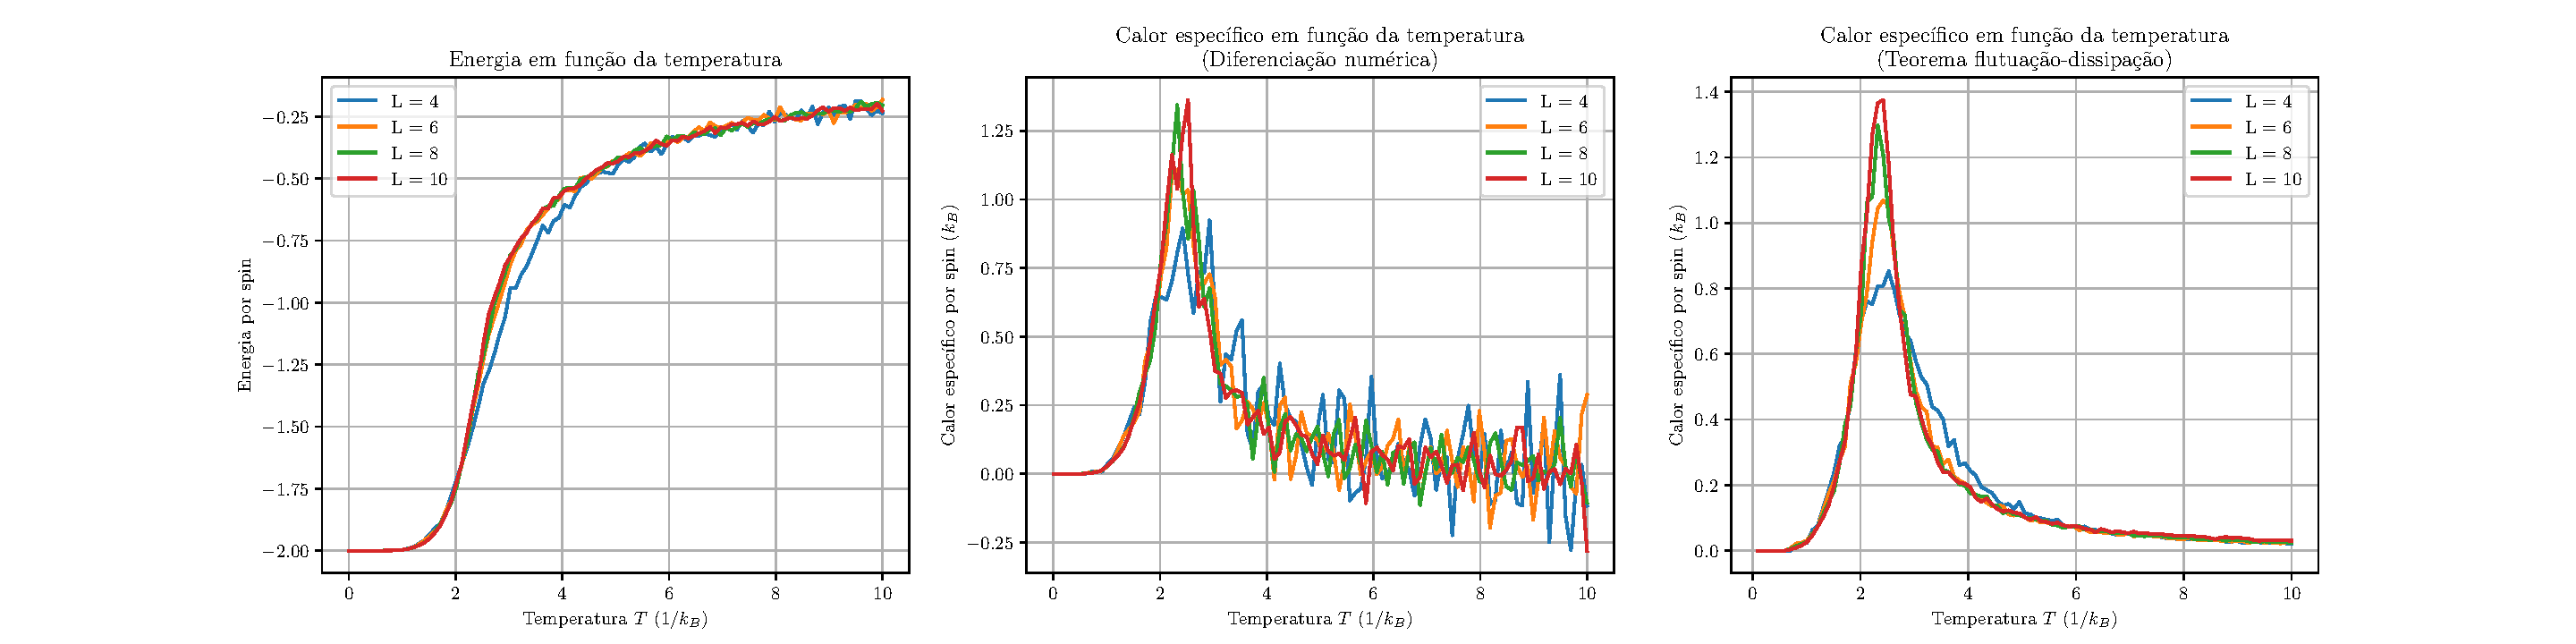
\includegraphics[width=\textwidth]{fig_2b.pdf}
        \caption{Gráfico do calor específico em função da temperatura para redes de diferentes tamanhos.}\label{fig2b}
    \end{figure}

    Pelos gráficos do meio e da direita na figura \ref{fig2b}, o resultado obtido por diferenciação númerica é muito mais ruidoso do que aquele obtido pelo teorema flutuação-dissipação.


\newpage
\subsection*{2.c)}

    Estimei as temperaturas críticas obtendo a temperatura do calor específico (pelo método da flutuação-dissipação) máximo nos gráficos do item anterior.
    Os resultados, na tabela \ref{tabTc}, são quase metade daquele obtido pelo método do campo médio.

    \begin{table}[ht]
        \centering
        \begin{tabular}{c|c}
            \( L \) & \( T_c \) (\( 1 / \kB \)) \\
            \hline
            4 & \num{2.53} \\
            6 & \num{2.42} \\
            8 & \num{2.32} \\
            10 & \num{2.42}
        \end{tabular}
        \caption{Tabela contendo os valores de temperaturas críticas para diferentes tamanhos de rede.}
        \label{tabTc}
    \end{table}

\newpage
\subsection*{2.d)}

    \begin{figure}[ht]
        \centering
        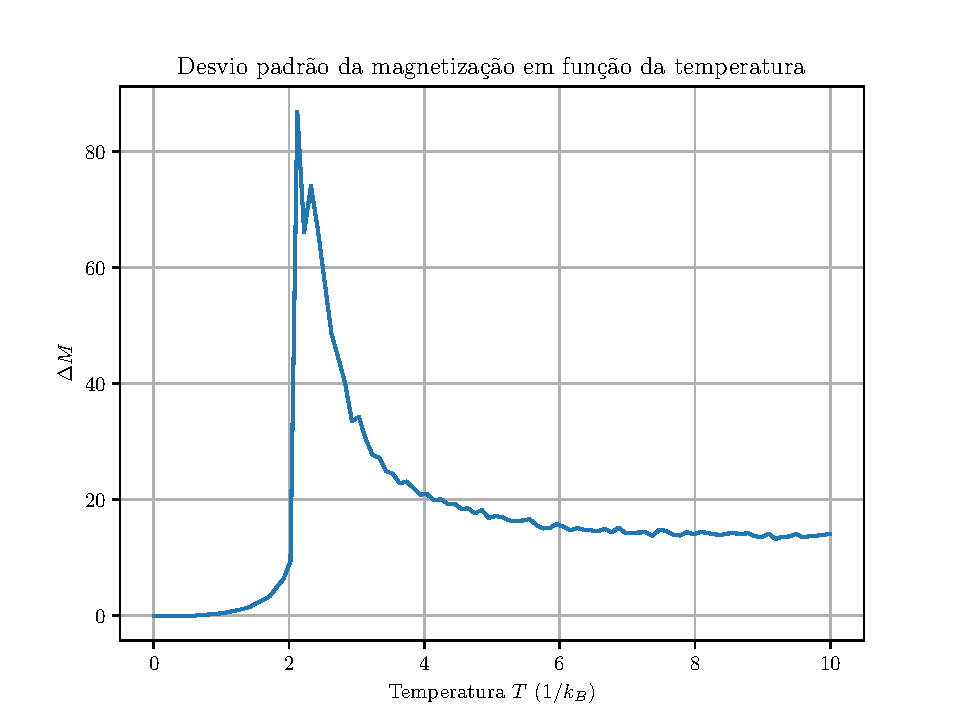
\includegraphics[width=0.7\textwidth]{fig_2d.pdf}
        \caption{Gráfico do desvio padrão da magnetização em função da temperatura.}\label{fig2d}
    \end{figure}

    Como o desvio padrão da magnetização tembém uma singularidade em torno dos mesmos valores de temperatura que os ítens anteriores, também podemos obter a temperatura crítica a partir desse gráfico.
    Estimei a temperatura crítica como a temperatura do desvio padrão máximo.
    Assim obtive \( T_c = \num{2.12} \).
    Esse valor é pouco menor do que os obtidos no ítem anterior.


\end{document}
